\documentclass[conference]{IEEEtran}
\usepackage[top=3cm, bottom=2cm, left=2cm, right=2cm, columnsep=20pt]{geometry}
\usepackage{pdfpages}
\usepackage{graphicx}
\usepackage{etoolbox}
\apptocmd{\sloppy}{\hbadness 10000\relax}{}{}
% \usepackage[numbers]{natbib}
\usepackage[T1]{fontenc}
\usepackage{ragged2e}
\usepackage[french]{babel}
\usepackage{listings}
\usepackage{color}
\usepackage{soul}
\usepackage[utf8]{inputenc}
\usepackage[export]{adjustbox}
\usepackage{caption}
\usepackage{amsmath}
\usepackage{amssymb}
\usepackage{float}
\usepackage{csquotes}
\usepackage{fancyhdr}
\usepackage{wallpaper}
\usepackage{siunitx}
\usepackage[indent]{parskip}
\usepackage{textcomp}
\usepackage{gensymb}
\usepackage{multirow}
\usepackage[hidelinks]{hyperref}
\usepackage{abstract}
% \renewcommand{\abstractnamefont}{\normalfont\bfseries}
% \renewcommand{\abstracttextfont}{\normalfont\itshape}
\usepackage{titlesec}
% \titleformat{\section}{\large\bfseries}{\thesection}{1em}{}
% \titleformat{\subsection}{\normalsize\bfseries}{\thesubsection}{1em}{}
% \titleformat{\subsubsection}{\normalsize\bfseries}{\thesubsubsection}{1em}{}

\usepackage{xcolor}
\definecolor{codegreen}{rgb}{0,0.6,0}
\definecolor{codegray}{rgb}{0.5,0.5,0.5}
\definecolor{codepurple}{rgb}{0.58,0,0.82}
\definecolor{backcolour}{rgb}{0.95,0.95,0.92}
\lstdefinestyle{mystyle}{
    backgroundcolor=\color{backcolour},   
    commentstyle=\color{codegreen},
    keywordstyle=\color{magenta},
    numberstyle=\tiny\color{codegray},
    stringstyle=\color{codepurple},
    basicstyle=\ttfamily\footnotesize,
    breakatwhitespace=false,         
    breaklines=true,                 
    captionpos=b,                    
    keepspaces=true,                 
    numbers=left,                    
    numbersep=5pt,                  
    showspaces=false,                
    showstringspaces=false,
    showtabs=false,                  
    tabsize=2
}
\lstset{style=mystyle}

\usepackage[most]{tcolorbox}
\newtcolorbox{note}[1][]{
  enhanced jigsaw,
  borderline west={2pt}{0pt}{black},
  sharp corners,
  boxrule=0pt, 
  fonttitle={\large\bfseries},
  coltitle={black},
  title={Note:\ },
  attach title to upper,
  #1
}

%----------------------------------------------------

\setlength{\parindent}{0pt}
\DeclareCaptionLabelFormat{mycaptionlabel}{#1 #2}
\captionsetup[figure]{labelsep=colon}
\captionsetup{labelformat=mycaptionlabel}
\captionsetup[figure]{name={Figure }}
\captionsetup[table]{name=Tableau}
\newcommand{\inlinecode}{\normalfont\texttt}
\usepackage{enumitem}
\setlist[itemize]{label=\textbullet}

\begin{document}

%----------------------------------------------------
\title{Écran tactile acoustique\\
\large Travail préparatoire \\
PHS3910 -- Techniques expérimentales et instrumentation\\ 
Équipe L3}

\author{\IEEEauthorblockN{Émile Guertin-Picard}
\IEEEauthorblockA{2208363}
\and
\IEEEauthorblockN{Maxime Rouillon}
\IEEEauthorblockA{2213291}
\and
\IEEEauthorblockN{Marie-Lou Dessureault}
\IEEEauthorblockA{2211129}
\and
\IEEEauthorblockN{Philippine Beaubois}
\IEEEauthorblockA{2211153}
}

\maketitle

\section{Introduction}
Dans le cadre du cours PHS3910, l'équipe est mandatée de conceptualiser
un piano tactile à l'aide du principe de retournement temporel. Avant
de développer le produit final, il faut premièrement simuler le fonctionnement 
du piano à l'aide de l'outil k-Wave, afin de déterminer les caractéristiques qui 
optimiseront sa performance. En variant la forme, le matériau de 
la plaque ainsi que la position du capteur directement dans la simulation,
une solution complète préliminaire peut être établie. Le choix de la solution finale est
principalement basé sur les concepts de résolution et de contraste.

Les choix retenus suite aux tests de simulation sont les suivants: une plaque
asymétrique avec trous, en \textcolor{red}{(À déterminer)}, avec un capteur situé \textcolor{red}{(À déterminer)}.
Le rapport ci-présent détaillera la méthodologie utilisée afin d'obtenir 
une étude statistique de la résolution et du contraste en fonction des
caractéristiques du piano, présentera les valeurs résultantes et leurs incertitudes 
respectives, et discutera des éléments pouvant être déduis de ceux-ci et implémentés 
dans la conception. Une présentation des prochaines étapes nécessaires à la complétion
du mandat sera aussi détaillée.

\section{Méthodes \label{methodes}}
%Garder en tête qu'on veut ''On vous demande de déterminer et de 
%faire une étude systémique et rigoureuse des paramètres
%principaux à optimiser. ''

%''piano tactile le plus près possible d’un piano acoustique''

%Méthodes : Transformer cette question dans un langage mathématique, 
%décrire les méthodes de simulations
Étant donné que le problème à considérer est de trouver les paramètres 
optimaux à l'aide d'une simulation, les méthodes de simulations sont décrites
en fonction des étapes importantes du programme MatLab.
Les formes des plaques considérées ont été choisies pour avoir un éventail de 
géométries (carré, cercle, forme asymétrique, avec et sans trous). 
Cela permet de voir l'impact de la symétrie et l'avantage attendu des asymétries. 
Du bois, du plexiglas et des métaux ont été testés pour voir l'impact de la 
vitesse du son dans le milieu sur le contraste et la résolution. 
Plus d'attention a été portée sur les métaux, sachant déjà que les matériaux plus 
denses et moins élastiques sont favorables à  la transmission d'ondes acoustiques 
\textcolor{red}{ajouter reference}.

Le signal obtenu à un récepteur à un endroit \textit{i} est modélisé comme la réponse 
impulsionnelle de la configuration (géométrie et matériau) à une impulsion d'une source
à un endroit \textit{j}. 
Pour chaque configuration, au lieu de simuler un émetteur pour un grand nombre de 
positions, il a plutôt été convenu d'effectuer la simulation d'un seul emplacement 
et d'utiliser le principe du retournement temporel. 
Ce principe permet d'interchanger les rôles de récepteur et d'émetteur. 
Ainsi, un seul impact a eu besoin d'être simulé à un endroit arbitraire en évaluant 
le signal reçu à une multitude de récepteurs distribués sur la plaque. 
À la suite du retournement temporel, les positions \textit{i} et \textit{j} 
sont intervertis. 
Pour chaque source, le signal reçu \textit{$S_j$} devient:
\[S_j(t)=h_{P_jS}(-t).\]
Une fois que la réponse impulsionnelle a été obtenue pour tout emplacement désiré sur la plaque, il a 
fallu en calculer la corrélation pour déterminer la résolution et le constraste de la
configuration. 
Pour réduire le temps de simulation, les retards accumulés sur chaque signal ont été 
retirés en gardant seulement une fenêtre de la réponse impulsionnelle. 
Les signaux inversés et recadrés ont été stockés et enregistrés pour pouvoir s'y référer 
lors du calcul de la corrélation. 
Une bande d'intérêt sur la plaque a également été choisie pour réduire le temps de 
calcul. 
Pour chaque émission de la bande, la corrélation entre le signal de cette émission et
de celui des autres émissions de la bande a été calculée. 
Ceci a permis de contruire un graphique 2D de la corrélation en fonction de la position pour un
nombre d'impulsions de la bande. 

Pour effectuer une analyse statistique de la résolution et du contraste, il a fallu 
faire correspondre une courbe gaussienne sur chaque graphique 2D obtenu précédement. 
La largeur à mi-hauteur de la gaussienne a pu déterminer la résolution alors que la 
différence entre le maximum de la courbe et le niveau du bruit a pu déterminer le contraste.
Les valeurs finales et leur incertitude respective découlent des impulsions choisies pour 
les graphiques; la moyenne et l'écart-type pour chaque variable sont calculées.




%Étapes (AU PASSÉÉÉ!!)
%1- Créer les configurations (Matériau + Géométrie)
%2- Simuler un impact à un endroit avec K-wave
%3- Évaluer le signal pour des récepteurs positionnés partout sur le matériau
%4- Faire un retournement temporel sur tous les signaux. Ce processus fait des récepteurs les émetteurs, et de l'émetteur le récepteur de chaque émission
%5- Éliminer les retards à l'aide d'une fonction fenêtre/rectangle pour accélérer la comparaison des signaux
%6- Pour gagner du temps, on choisi une bande d'intérêt de la plaque où on sélectionne les émissions une à la fois. 
%7- Pour chaque émission, on la compare à toutes les émissions enregistrées de la bande, formant un graphique 2D de la corrélation en fonction de la position
%8- Une fois chaque émission de la bande d'intérêt testée, on a effectué une étude statistique de la résolution et du constraste en ''fittant'' une gaussienne sur le graphique 2D. 

%9 Faire la moyenne de plusieurs résolution et contraste pour obtenir l'incertitude statistique




\section{Résultats}
%Résultats choisis, obtenus à l’aide des Méthodes et permettant d’informer la Discussion.
%Attention, ici, les résultats doivent être décrits de façon factuelle, mais ne doivent
% pas être discutés.
%Typiquement des figures et des tableaux seront utilisés et le texte décrira de façon 
%neutre les aspects importants des tableaux et figures à remarquer. Des incertitudes 
%sur tous les résultats sont attendues. 
%Plus d’attention devra être portée aux variables qui ont un effet (positif ou négatif) 
%et moins d’attention sera portée aux variables n’ayant pas ou peu d’effet.

Les géométries d'un carré, d'un cercle et d'un rectangle avec des trous sont à être 
testées. 
La première géométrie testée est celle d'un carré de 32 pixels de côté fait de bois 
qui est illustré à la figure \cite{fig:GéoCarré32}
\begin{figure}[h!]
  \centering
  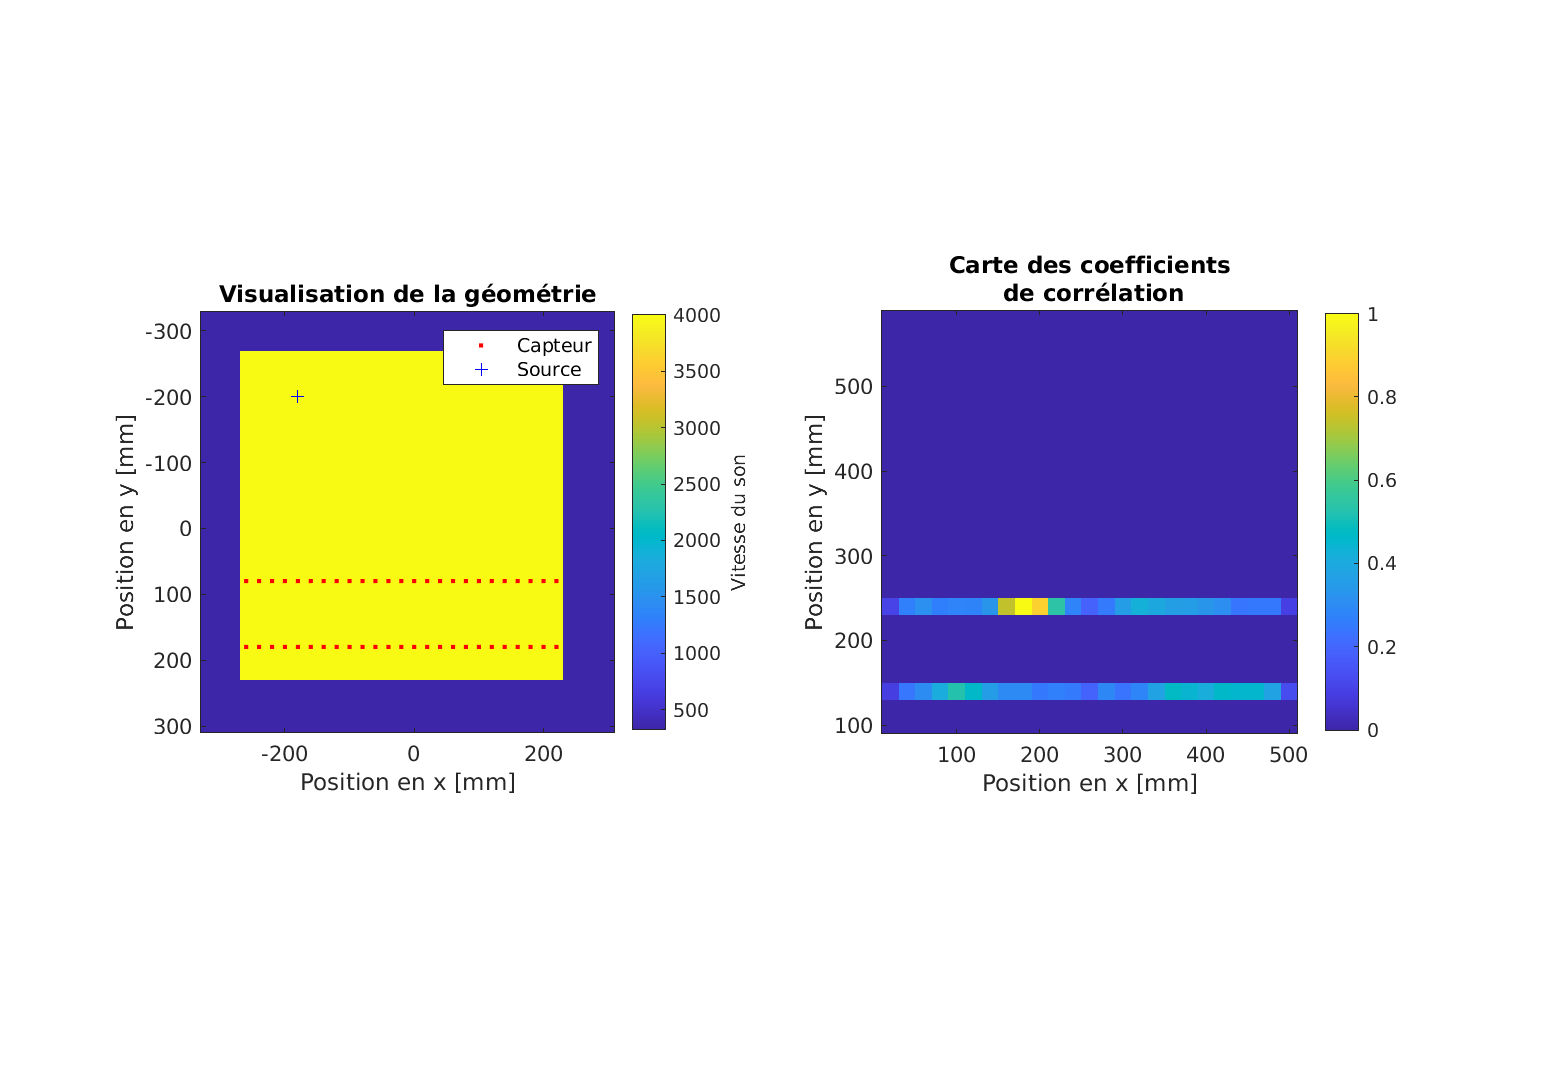
\includegraphics[width=0.4\linewidth]{Géométire carrée et double bande.png}
  \caption{Illustration de la plaque 32X32 avec les positions du récepteur marqué 
  d'une croix et des sources marquées d'un point ainsi que la corrélation obtenue
  entre le signal provenant du point jaune et celui de chaque autre point}
  \label{fig:GéoCarré32}
\end{figure}

%Décrire le graphique de corrélation en fonction de la positon, avec 
%L'endroit où c'est plus corrélé et comment proche c'est un peu corrélé aussi
%Décrire la graphique où on voit la géométrie avec l'emplcement du capteur et
%des sources
%Décrire le graphique de gaussienne rapidement


\begin{figure}[h!]
  \centering
  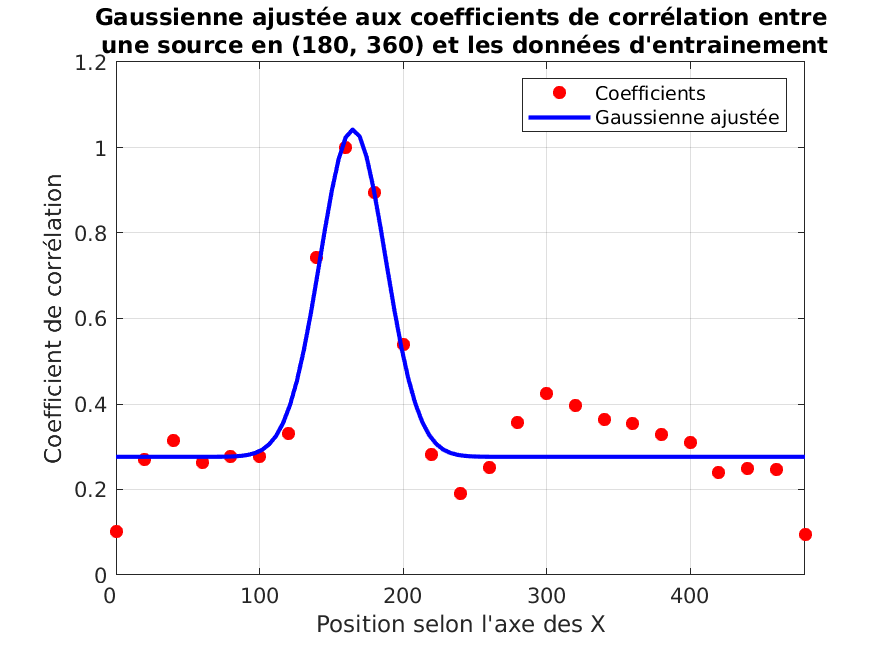
\includegraphics[width=0.4\linewidth]{Gaussienne fit 1 point.png}
  \caption{Graphique du fit gaussien}
  \label{fig:GaussCarré32}
\end{figure}

Le contraste obtenu est de ($0,7023 \pm 0,0121$) pixels, ce qui correspond à une 
incertitude relative d'environ 2\%.
%Quelle est l'unité ici?
La résolution obtenu pour cette géométrie est de ($2,6921 \pm 0,1353$) pixels. 
L'incertitude relative de la résolution est d'environ 5\%. 

Les résultats de la résolution et du contraste sont montrés dans le graphique 
\cite{rés-con} dans lequel les configurations préférables sont situées vers le 
coin supérieur droit. 
%Graphique de la résolution vs le contraste, avec le type de matériau donné par
%la couleur, la géométrie donnée par la forme du point et les infos de résolution
%et contraste données par la position sur la graph

%Parler de quels paramètres affectent plus le contraste et la résolution!!

\section{Discussion}
Ayant obtenu un fit 2D gaussien, il est possible d'analyser et de comparer les variables pertinentes, 
le contraste et la résolution, selon différents paramètres physiques qui ont été élaborés dans la section \ref{methodes}.
Le graphique \ref{} offre un échantillon des résultats obtenus pour une plaque carrée, sans trous et 
en bois. En ayant utilisé le retournement temporel, la durée de simulation a pu être réduite, ce qui a 
permis d'obtenir des réponses temporelles pour un nombre d'échantillons considérablement plus grand. 
Cette décision a permis d'améliorer la définition des fits gaussiens. Six échantillons ont été choisis au
hasard parmi les deux bandes considérées, offrant un poids statistique aux résultats assez important.

En observant le graphique \ref{}, on peut noter que l'emplacement de la source du signal
correspond à une corrélation de 1. Ceci s'explique facilement par le fait que le signal choisi au
hasard comme source et le signal de référence sont les mêmes (le choix de réutiliser le signal a été fait encore
une fois pour réduire le temps de compilation). La courbe gaussienne a une correspondance quasi parfaite pour les données
proches du maximum du pic, mais réduit en terme d'exactitude pour les données au niveau de la base
de la gaussienne.

Les résultats obtenus avec cette simulation permettent d'avoir un aperçu quant-aux
résultats possibles des simulations de d'autres paramètres. Le cas le plus favorable suite à 
un plus grand nombre de simulations serait d'avoir une résolution faible
et un contraste important. En évaluant l'allure de la courbe pour le cas ci-présent, on peut estimer
qu'il serait souhaitable de trouver des paramètres offrant un contraste plus grand que ceux évalués ici.
La résolution, quant-à-elle, semble déjà suffisament bonne. Évidemment, il est difficile d'arriver à une 
conclusion pertinente sans d'autres éléments de comparaison.



\clearpage

% \bibliographystyle{unsrtnat}
% \bibliography{My_Library}

\end{document}
